% Carattere dimensione 12
\documentclass[12pt,openany]{report}

\setlength{\parindent}{0pt}

% Per la stampa fronte-retro sostituire con:
% \documentclass[12pt, twoside]{report}

% Margini (4cm a sx, 2.5cm a dx, 2.5cm in alto, 2.5cm in basso)
\usepackage[top=2.5cm, bottom=2.5cm, left=2.5cm, right=2.5cm, centering]{geometry}

% Per la stampa fronte-retro sostituire con: 
% \usepackage[top=2.5cm, bottom=2.5cm, inner=4cm, outer=4cm, right=2.5cm, centering]{geometry}

% Interlinea
\linespread{1.5}

% Librerie utili
\usepackage[english]{babel} % applicazione regole di scrittura per la lingua italiana 
\usepackage[utf8]{inputenc} % codifica UTF-8
\usepackage{scrlayer-scrpage} % stili pagina per il frontespizio
\ifoot[]{}
\cfoot[]{}
\cfoot[\pagemark]{\pagemark}
\pagestyle{scrplain}
\usepackage{mathptmx} % font Times New Roman (simile)
\usepackage{graphicx} % inserimento di immagini
\usepackage{csquotes} % per le citazioni "in blocco"
\usepackage[backend=biber, sorting=none, ]{biblatex} % bibliografia con pacchetto biblatex (https://ctan.org/pkg/biblatex?lang=en)
\addbibresource{bibliography.bib}
\appto{\bibsetup}{\raggedright}

\usepackage{titlesec} % per la formattazione dei titoli delle sezioni, capitoli etc.
\usepackage{float} % per il posizionamento delle immagini

\usepackage{listings} % per il codice di programmazione
% Fonte https://en.wikibooks.org/wiki/LaTeX/Source_Code_Listings. Per la lista di sintassi riconosciute.
\renewcommand{\lstlistingname}{Code}% Listing -> Codice
\usepackage{xcolor}  % stile del codice
\definecolor{mygreen}{rgb}{0,0.6,0}
\definecolor{mygray}{rgb}{0.5,0.5,0.5}
\definecolor{mymauve}{rgb}{0.58,0,0.82}
\definecolor{darkgray}{rgb}{.4,.4,.4}
\definecolor{navy}{HTML}{000080}
\definecolor{purple}{rgb}{0.65, 0.12, 0.82}
\definecolor{codepurple}{rgb}{0.58,0,0.82}
\definecolor{backcolour}{rgb}{0.95,0.95,0.92}

% \usepackage{longtable}
\usepackage{tabularx}
\usepackage{ragged2e}



% Stili configurabili del codice (lslisting) 
\lstset{ %
belowcaptionskip=0.5em,
backgroundcolor=\color{backcolour}, % choose the background color; you must add \usepackage{color} or \usepackage{xcolor}
basicstyle=\footnotesize, % the size of the fonts that are used for the code
breakatwhitespace=false, % sets if automatic breaks should only happen at whitespace
breaklines=true, % sets automatic line breaking
captionpos=b, % sets the caption-position to bottom
commentstyle=\color{mygreen}, % comment style
deletekeywords={...}, % if you want to delete keywords from the given language
escapeinside={\%*}{*)}, % if you want to add LaTeX within your code
extendedchars=true, % lets you use non-ASCII characters; for 8-bits encodings only, does not work with UTF-8
frame=single, % adds a frame around the code
keepspaces=true, % keeps spaces in text, useful for keeping indentation of code (possibly needs columns=flexible)
keywordstyle=\color{codepurple}, % keyword style
% language=Octave, % the language of the code
morekeywords={*,...}, % if you want to add more keywords to the set
numbers=left, % where to put the line-numbers; possible values are (none, left, right)
numbersep=5pt, % how far the line-numbers are from the code
numberstyle=\tiny\color{mygray}, % the style that is used for the line-numbers
rulecolor=\color{black}, % if not set, the frame-color may be changed on line-breaks within not-black text (e.g. comments (green here))
showspaces=false, % show spaces everywhere adding particular underscores; it overrides 'showstringspaces'
showstringspaces=false, % underline spaces within strings only
showtabs=false, % show tabs within strings adding particular underscores
stepnumber=1, % the step between two line-numbers. If it's 1, each line will be numbered
stringstyle=\color{mymauve}, % string literal style
tabsize=2, % sets default tabsize to 2 spaces
title=\lstname % show the filename of files included with \lstinputlisting; also try caption instead of title
}


% END of listing package

\makeatletter
\renewcommand{\chapter}{%
  \thispagestyle{plain}% Optional: Adjust page style
  \global\@topnum\z@
  \@afterindentfalse
  \secdef\@schapter\@schapter}
\makeatother

% Formato delle intestazioni
\titleformat{\chapter}[hang]
  {\normalfont\LARGE\bfseries}{\thechapter.}{0.5em}{\LARGE}
\titlespacing*{\chapter}{0pt}{30pt}{25pt}

\newcommand{\firstchapter}{
  \titlespacing*{\chapter}{0pt}{0pt}{25pt} % Reduce space before first chapter title
}

\begin{document}
\justify

\setcounter{page}{1}
\addtocontents{toc}{\protect\thispagestyle{empty}}
\addcontentsline{toc}{chapter}{Introduction} % Capitolo non numerato

%header (da migliorare)
EMOTION DETECTION IN SONG LYRICS STANZAS\\
TEXT ANALYTICS - A.Y. 2024/2025\\
Group 2 - Barbieri, Bosco, Ferrara, Rotellini, Zizza


% Abstract section
\firstchapter
\chapter*{Abstract}
\label{ch:abstract}
Lyrics serve as one of the main foundations of songs, playing a crucial role in expressing feelings in many different ways.
The emotional tone of songs can also serve various purposes, such as automatized playlist creation or songs' organization,
offering an alternative to the more traditional genre-based classification. This study focuses on developing four Machine Learning models
to classify emotions conveyed in English song lyrics, at the stanza level.
The models were chosen for their proven effectiveness across various domains and
their diverse approaches, providing a thorough investigation of different
techniques and depths for emotion classification in text.\\
The study begins with the preprocessing of the \textit{Genius Song Lyrics}\textsuperscript{\cite{geniusdataset}} dataset.
% This was a deep and time-consuming process, which ultimately resulted in a complete reshape of the originale dataset. 
The models were then trained through transfer learning, by generating the ground
truth using the already existing ALBERT Base v2 model.
% The ground truth was created with an already existing model: Albert Base v2, which was chosen to avoid the computational costs of larger models like BERT. The resulting labelled dataframe was then splitted following the train/test split protocol.
% The study proceeded with the training and the performance analysis of the following models: Random Forest and Support Vector Machine, followed by a One-Dimensional Convolutional Neural Network and a Recurrent Neural Network. 
The results are discussed to highlight the specific challenges encountered.
% \section*{Abstract}
% Analyzing the emotional tone of songs texts can give insights into
% societal trends and this information can be useful especially for recommendation
% algorithms.
% This study aims to build 4 Machine Learning models that classify
% emotions expressed in English song lyrics at the stanza level; 
% the emotion labels are given according to
% Plutchik's 8 primary emotions.

% Introduction (on the same page)
\chapter*{Introduction}
\label{ch:Introduction}
Lyrics serve as one of the main foundations of songs, playing a crucial role in
expressing feelings in many different ways.
The emotional tone of songs can serve various purposes, such as
automatized playlist creation or songs' organization,
offering an alternative to the more traditional genre-based classification. \\
%Analyzing the emotional tone of song texts can give useful insights about individual mental states, cultural trends, social issues and more.
% The main goal of this project is to perform emotion detection on stanzas of songs.
% The goal of this project is the development of 4 Machine Learning models
% that perform emotion detection on songs' stanzas.
To obtain a deeper understanding of emotional fluctuations within the texts,
the models assign emotion labels to individual stanzas instead of full songs.
The emotion labels correspond to Robert Plutchik's eight primary emotions
(shown in figure~\ref{fig:primary_emotions}), providing a comprehensive range
for representing various emotional states.\\
\begin{figure}[H]
    \centering
    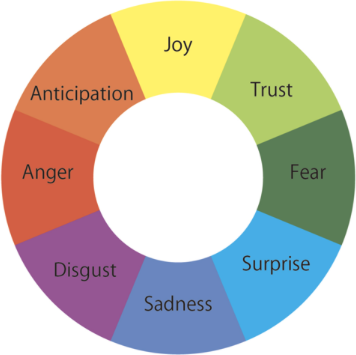
\includegraphics[scale= 0.25]{pictures/plutchik_primary_emotions.png}
    \caption{Plutchik's eight primary emotions}
    \label{fig:primary_emotions}
\end{figure}

This report aims to clearly cover and illustrate various aspects of the work. 
The \textit{Methods} chapter contains a detailed explanation of the data and
procedures used in the project, providing descriptions of each part implemented
in the project.
The \textit{Results} chapter presents an overview of the
obtained outcomes.
These results are further explored in the final sections, \textit{Discussion}
and \textit{Conclusions}, which interpret the general findings, recap the
primary objectives of the work, and discuss the importance or potential
applications of the results.


% Dataset overview
% !!! cut, content in intro
% % !!!
% cut at the moment; content moved to introduction

\chapter{Dataset overview}
\label{ch:capitolo1}

% copy-pasted from project proposal
The dataset utilized in this project represents a subset of songs
derived from the Genius Song Lyrics Dataset\textsuperscript{\cite{geniusdataset}}.
The dataset contains 11 attributes
that represent various song data, including the lyrics.
The original dataset includes songs in all languages: for our aim
we will be using the english ones only.\\

The dataset doesn't have emotion labels, which are essential for training the models.
To create the ground truth, the model
Albert Base v2\textsuperscript{\cite{albert-base-v2}} was used, classifying
stanzas' lyrics with Plutchik's eight primary emotions.

% The stanzas are labeled using Robert Plutchik's 8 primary emotions;
% the emotions included in this representation are:
% anger, fear, sadness, disgust, surprise, anticipation, trust, and joy.
% Such multifaceted emotions allow us to finely analyze the feelings and
% moods conveyed by songs.
% 
% \clearpage

%  "METHODS" 
\chapter*{Methods}
\label{ch:capitolo2}
The dataset used in this project is a sampled subset of English-language
songs derived from the \textit{Genius Song Lyrics Dataset}\textsuperscript{\cite{geniusdataset}}.
The original dataset contained numerous attributes; the ones considered
relevant for model training are:
\begin{itemize}
    \item \textbf{title:} the song's title;
    
    \item \textbf{lemmatized\_stanzas:} lyrics of the single stanza;
    
    \item \textbf{stanza\_number:} identifies the position of the stanza in the song;

    \item \textbf{is\_chorus:} boolean variable that attests whether the stanza is
        a chorus or not;
    
    \item \textbf{is\_country, is\_pop, is\_rap, is\_rb, is\_rock:} boolean variables, result of a one-hot encoding process, that represent songs genres;

    \item \textbf{label:} represents the emotional classification of the stanza,
        assigned by Albert Base v2\textsuperscript{\cite{albert-base-v2}}.
\end{itemize}
All of these attributes, except for \texttt{title}, were the result
of the preprocessing phase, as described in section~\ref{preprocessing}.
Due to limited computational power, the labeling process was time-intensive,
ultimately resulting in a limited dataset, with a few more than 100.000 entries.

%PREPROCESSING
\section*{Preprocessing}
\label{preprocessing}
The preprocessing phase began by sampling the dataset while maintaining genre
distribution. Text cleaning focused on removing irrelevant noise, such as
square-bracketed items, and splitting lyrics into individual stanzas using
stanza-related keywords (e.g., "chorus", "verse").
Uninformative stanzas, such as empty or very short ones, were discarded,
resulting in a dataset of numbered stanzas.
A boolean feature, \texttt{is\_chorus}, was added to mark repeated or chorus-related
stanzas, and duplicate stanzas were removed to eliminate redundancy.
Further cleaning involved removing stanza headers and newline characters,
producing cleaner stanzas for labeling.
Lemmatization was performed using the \texttt{spaCy} library, generating
tokenized stanzas by filtering out punctuation. ALBERT Base v2 was then
fine-tuned to label approximately 100,000 stanzas with emotional categories.
A preliminary class distribution analysis showed a slight imbalance, with
\textit{joy} being the most frequent (18\%) and \textit{disgust} the least (10\%).
Figure~\ref{fig:enter-label} illustrates the distribution across all classes.


% The initial preprocessing step involved sampling from the original dataset
% while maintaining the proportional distribution of genres.
% This approach ensured that the genre representation in the sampled subset
% accurately reflected that of the full dataset.\\

% The preliminary text cleaning process focused on the \texttt{lyrics} attribute,
% which contained the complete lyrics of each song in string format.
% Initially, a regular expression (RegEx) was built to remove noise from the
% lyrics, specifically targeting words enclosed in square brackets that were
% irrelevant to the stanza splitting process. Many keywords marking different
% stanzas were written within square brackets, and removing non-keyword items
% inside brackets was crucial to avoid potential issues.\\

% The next critical step was stanza splitting. After cleaning texts from
% noisy square-bracketed items, lyrics were split based on various keywords
% used to denote stanzas (such as "chorus", "verse", "intro", "outro", "refrain", "hook", etc.).
% The RegEx developed accounted for the different formats in which these keywords
% appeared, including square brackets, parentheses, or no brackets at all, as well
% as stanzas separated only by double newline characters.
% The output of this step was, for each song record, a list of strings
% representing individual stanzas (each stanza has also a header with the corresponding
% keyword; this aspect will be discussed in the next paragraph).
% Next, uninformative strings—such as empty strings or those with fewer
% than 20 characters—were removed, as they were too short to provide meaningful
% content.
% As a result, the output of this preliminary preprocessing phase was a dataset
% where the records were no longer whole songs but individual stanzas, each
% numbered according to its position within the song.\\

% A further and more detailed cleaning process on the stanzas involved the creation
% of the boolean feature \texttt{is\_chorus}, which was assigned a \texttt{true}
% value for repeated stanzas within the same song or for stanzas with headers such
% as "hook", "chorus", "refrain", or "bridge".
% Next, stanza headers and newline characters between verses were removed to obtain
% cleaner stanzas.
% Since choruses, hooks, bridges, and refrains often repeat throughout songs,
% duplicate stanzas were discarded to avoid redundant data. This resulted in a
% dataset of cleaned, non-duplicate stanzas, which served as the checkpoint for
% the labeling step and the starting point for the text lemmatization process.\\

% The subsequent step involved lemmatizing the stanzas using the \texttt{spaCy}
% library. A list of lemmatized tokens was created by filtering out punctuation
% and empty words. Lemmatization was chosen over stemming because it produces
% more accurate and meaningful results, particularly for tasks requiring semantic
% understanding, such as the one at hand.\\

% Since the dataset was not pre-labeled at the stanza level, ALBERT Base v2 was employed for this task.
% This transformer model is specifically designed to be fine-tuned on tasks that
% require an understanding of the entire sentence, such as sequence classification. As specified above, due to computational issues the labeling was performed on around 100'000 stanzas. 
% A preliminary analysis of the distribution of the classes revealed a slight disparity in representation among the labels, which is expected in this scenario. 
% The most represented class was \textit{joy}: around 18\% of the total number of texts were classified as such, followed by \textit{fear} and \textit{anger} at 14\% each. 
% The categories \textit{sadness}, \textit{trust}, \textit{anticipation} and \textit{surprise} each constituted 11\%, while \textit{disgust} was the least represented at 10\%. 
% Figure~\ref{fig:enter-label} shows the number of stanzas belonging to each label.
\begin{figure}[H]
    \centering
    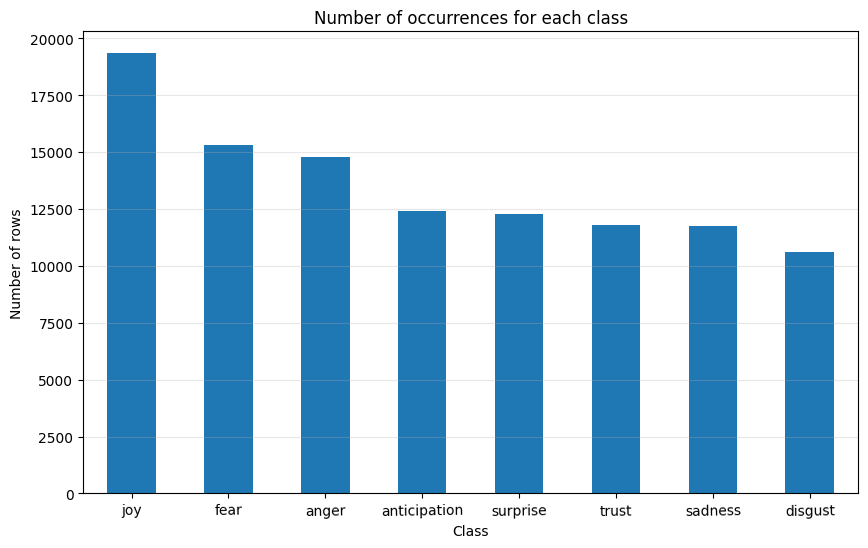
\includegraphics[width=0.7\linewidth]{pictures/exploratory_graph.png}
    \caption{Number of stanzas for each label}
    \label{fig:enter-label}
\end{figure}

\section*{Models}
The selected model architectures are:
\begin{itemize} 
    \item \textbf{Random Forest}: A robust ensemble learning method known for
    its ability to handle complex, high-dimensional datasets effectively.
    \item \textbf{Support Vector Machine (SVM)}: A powerful classifier that
    excels in separating classes by finding the optimal hyperplane,
    particularly effective in text classification tasks.
    \item \textbf{One-Dimensional Convolutional Neural Network (1D-CNN)}:
    Designed to capture local patterns in sequential data, leveraging
    convolutional layers to learn hierarchical features.
    \item \textbf{Recurrent Neural Network (RNN)}: Utilized for its strength
    in processing sequential data, with the ability to capture contextual
    relationships between words across different stanzas.
\end{itemize}
Their different approaches and depths are an important point of the study, as they
offer interesting insights into the possible different techniques and levels of
complexity required for detecting emotional tones in complex pieces of text.

%MODELLI STATICI
\subsection*{Static Models}
% The development of static models was then simple and straight forward.
% Static models are here meant to provide a performance comparison
% for the more complex Neural Networks.
% The two architectures are the same, consisting of a preprocessing
% layer to handle the inputs, followed by the classifier itself.\\

% The preprocessing layers handle both \texttt{title} and
% \texttt{lemmatized\_stanzas} through TF-IDF for feature extraction.
% An additional analysis aimed at identifying the most significant features for
% each emotion label in the dataset was conducted to enhance classification.
% Feature importance analysis was performed on the already labeled and
% lemmatized dataset, following these steps:
% \begin{itemize}
%     \item \textbf{Custom Stopword List Creation}: A custom stopword list was
%     compiled, consisting
%     of the most frequent and generic words in the dataset, along with additional
%     punctuation marks and common typographical errors not covered by the default
%     NLTK stopword lists.

%     \item \textbf{Stopword Removal}: Irrelevant words identified by the custom
%     stopword list were removed from the lemmatized stanzas to reduce noise in
%     the data.

%     \item \textbf{TF-IDF Analysis per Label}: A function was developed to
%     compute TF-IDF scores for a given text, with parameters \texttt{min\_df}
%     set to 2 and \texttt{max\_df} set to 0.80.
% \end{itemize}
% This configuration ensured that words appearing in fewer than two or
% more than 80\% of the documents were ignored, minimizing the influence of
% extremely rare or overly common words. The function was applied separately to
% the cleaned stanzas for each label, with the aim of identifying the most
% relevant features per emotion category.
% The results, however, did not meet expectations, though the outcome was not
% entirely surprising. Most labels shared at least two common features, and
% certain labels (such as surprise and trust) shared all features.
% Additionally, all identified features exhibited very low TF-IDF scores,
% below 0.05.
% This result appears to be inherent to the nature of the dataset: song lyrics
% frequently contain repetitive and generic language, making it difficult to
% distinguish specific emotions based solely on textual features.
% Consequently, the analysis was concluded at this point.\\

% Random Search was chosen for hyperparameter tuning, for both models.
% Cross validation is also used in order to provide a more accurate
% estimate of model performance.
The development of static models aimed at providing a performance benchmark for
more complex neural networks.
Both architectures consisted of a preprocessing layer, followed by a classifier.
The preprocessing handled title and \texttt{lemmatized\_stanzas} using TF-IDF for feature
extraction.\\

To improve classification, feature importance analysis was conducted on the
labeled dataset:
\begin{itemize}
    \item \textbf{Custom Stopword List Creation}: A custom list of frequent and generic words, punctuation, and common typographical errors was compiled.
    \item \textbf{Stopword Removal}: Irrelevant words were removed to reduce data noise.
    \item \textbf{TF-IDF Analysis per Label}: TF-IDF scores were computed for each emotion label, with parameters set to minimize the influence of overly common or rare words.
\end{itemize}
Despite these efforts, the analysis did not yield expected results, with most
labels sharing common features and low TF-IDF scores.
This was likely due to the repetitive and generic nature of song lyrics.\\

For hyperparameter tuning, Random Search and cross-validation were used to
estimate model performance more accurately.

\subsection*{Neural Networks}
The architectures were developed and tuned through empirical,
reiterated testing. These parameters helped with the process, and can
be used for further experimentation.
Both the Recurrent Neural Network and the One-Dimensional Convolutional
Neural Network share the same preprocessing
architecture. Most attributes are processed in the same manner as in
the Static Models; specific steps are applied to \texttt{lemmatized\_stanzas}
and \texttt{title}.
Non-Negative Matrix Factorization is applied to \texttt{title} in addition to
Term Frequency-Inverse Document Frequency
to extract latent topics, providing a richer representation of the
textual data.\\

\texttt{lemmatized\_stanzas} are handled by Convolutional and Recurrent
pipelines of the two Networks.
Elements are first tokenized, and then padded in order to
get an input with consistent shape, which is essential for both types of
recurrent layers.

\subsubsection*{One-Dimensional Convolutional Neural Network}
The Convolutional part of the architecture is specifically designed to extract and learn
local patterns in \texttt{embedding\_lyrics}.
Its structure consists of three convolutional layers, each applying filters of
varying sizes. This allows to detect patterns at different granularities.
These layers are followed by Global Max Pooling, to reduce the previous output's
dimension to a fixed-length vector, as well as retaining focus on the most
informative patterns.
A dropout layer is then applied, to introduce regularization and prevent
overfitting.

\subsubsection*{Recurrent Neural Network}
The Recurrent part of the architecture is specifically designed to extract and learn
local patterns in \texttt{embedding\_lyrics}.
Its structure consists of three Gated Recurrent Units (\texttt{GRU} layers)
to model temporal relationships. These are characterized by progressively smaller
numbers of units; this allows pattern capture at different abstraction levels.
All three layers in the architecture use the \texttt{tanh} activation function
to compute the hidden state and
the \texttt{sigmoid} activation function for the recurrent gate.
The first and second layers return the full sequence of hidden states for each
time step in the input sequence, enabling richer learning of patterns over time.
Dropout is applied on every layer, to prevent overfitting and add regularization.

\subsection*{Shared Components}
The remaining features are handled by a simple pipeline, which concatenates
their Input layers.
The inputs are passed them through a dense layer to create a compact
representation.
The output of the lyrics-processing branch is concatenated with the processed
additional features.
The combined representation is passed through a Dense layer with 32 units
(ReLU activation), followed by a Dropout layer with a rate of 0.3.
Finally, the output layer uses 8 units with a softmax activation, corresponding
to the classification into 8 emotion categories.\\


The models are trained using categorical cross-entropy as the loss function,
as it consistently produced better-performing results for both types of
neural networks.
As evaluation metric, the better performing one was categorical accuracy.
Other metrics were tested for evaluation purposes, particularly
top-k categorical accuracy with $k=2$, which yielded interesting insights
by considering a prediction correct if the true label is among the top two
predicted classes. While it showed potential in improving generalization and
preventing overfitting, it was ultimately discarded as a primary evaluation
metric. This is because, with $k=2$, the model has a 25\% baseline
chance of being correct when there are eight possible classes, which reduces
the precision required for accurate learning and limits performance improvements.\\

In addition to standard supervised learning, the script supports semi-supervised
learning. It can be utilized either strictly for transfer learning or in a data
augmentation approach. When using the data augmentation approach, the model's
weights can be reset prior to training on the newly pseudo-labeled data, allowing
for more robust retraining on an expanded dataset.
The results obtained 

%\clearpage

% static models
% \chapter{Static Models}
\label{ch:static_models}


\section{Random Forest}

\section{SVM}


% \clearpage

% neural networks
% \chapter{Neural Networks}
\label{ch:capitolo4}

\section{One-Dimensional Convolutional Neural Network}

\section{Recurrent Neural Network}

% \clearpage
\chapter*{Results}
\label{ch:results}
% The performances of the models were evaluated using the
% \texttt{classification\_report} function from the \texttt{scikit-learn} library. 
% This function is particularly useful as it offers an overview of key evaluation
% metrics commonly used in Machine Learning, i.e. accuracy, precision, recall,
% and F1-score.\\
The performance metrics taken into account for evaluation are the following:
accuracy, precision, recall, and F1-score. Taking all of them into account
is crucial to accurately evaluate how well each model performs.

For the static models implemented in this project, the classification report
revealed an accuracy of 34\% for the Random Forest algorithm and 43\% for SVM. 
These results can be considered reasonable, given that the task at hand is a
multi-class classification problem with 8 classes.\\

\textbf{AGGIUNGERE ALTRO}

\chapter*{Discussion}
\label{ch:discussion}

An interesting aspect of the explainability analysis is the visualization of the results.
The \textbf{left section} of the graph in Figure~\ref{fig:expl} displays the predicted probabilities for each class. In the \textbf{center section}
feature importances are ranked from most to least relevant and divided into two groups: on the right
features with a positive influence on the predicted label; on the left, those with a negative influence that suggest the model should consider other classes.
The \textbf{right section} of the graph highlights the values of the most important
features, using bright colors to indicate features with a positive influence on the prediction.

\begin{figure}[H]
    \centering
    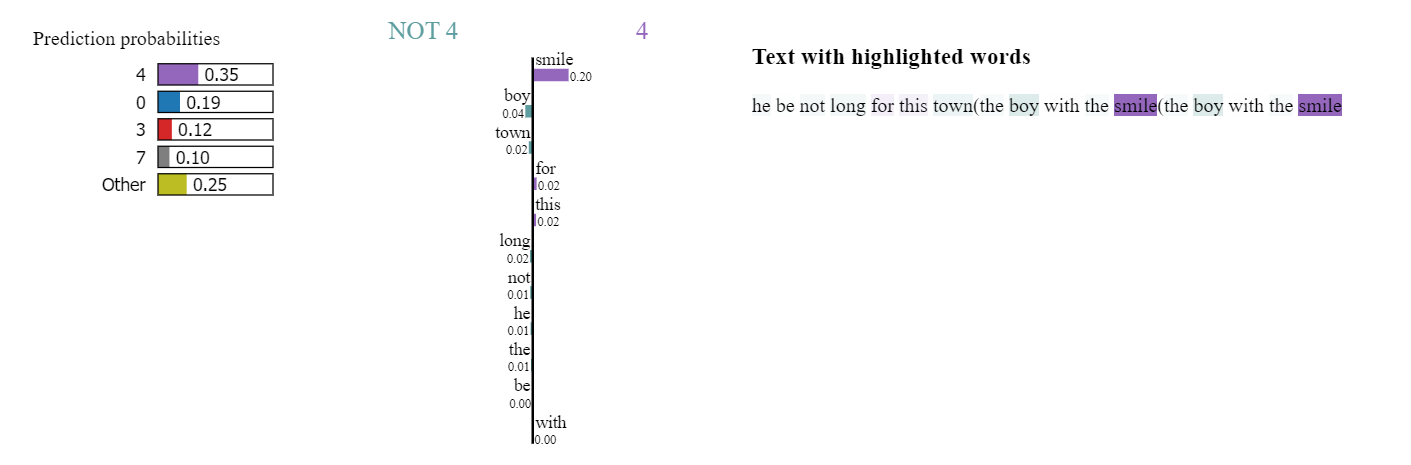
\includegraphics[scale= 0.55]{pictures/expl.png}
    \caption{Explainability - visualization}
    \label{fig:expl}
\end{figure}

The figure above illustrates a prediction where the model assigned the label \textit{joy} to the stanza under analysis, but the correct label, assigned by the ALBERT model (as mentioned in the \textit{Methods} section), was \textit{sadness}.
However, the word \textit{smile}, which is brighty highlighted, intuitively suggests that \textit{joy} might be a more plausible class for this stanza, even one that ALBERT could reasonably assign. 
This observation raises a critical issue: the transfer learning approach used to create the ground truth appears to have some limitations; in some instances the SVC model assigns a label that seems more contextually appropriate for the stanza, 
yet it differs from the supposedly correct label provided by ALBERT.\\

This phenomenon may also explain the results presented in the figures from the
previous chapter.
However, it is not the only plausible explanation; notably, the poor performance
could be attributed to a general overlap of features.
By applying a filter to exclude the most common words, it's possible that the
remaining words carry less ambiguous emotional meanings, and are easier to interpret.
% TODO quote figures



%DISCUSSIONS AND CONCLUSION
\chapter*{Conclusions}
\label{ch:conclusions}

\textbf{AGGIUNGERE INFO SPECIFICHE AL PROGETTO}\\

In conclusion, this study aimed at demonstrating how emotion detection in song lyrics stanzas can provide valuable insights into the emotional landscape of music and how it can be implemented with Machine Learning models. 
These findings have practical applications, such as improving music recommendation systems and creating mood-based playlists. 
At the same time, the study faced challenges, particularly with interpreting ambiguous or context-dependent lyrics, which highlights opportunities for further research in this field.


\section*{Future developments}
\clearpage

% \renewcommand{\contentsname}{Bibliography}
% \bibliographystyle{plain}
% \bibliography{bibliography}
% \addbibresource{bibliography.bib}
\printbibliography
\renewcommand{\listfigurename}{List of figures}
\listoffigures

% \thispagestyle{empty}
% \clearpage


\end{document}